\documentclass{article}
\usepackage{geometry}
\geometry{
  a4paper,
  left=30mm,
  right=30mm,
  top=20mm
}
\setlength{\parindent}{0pt}
\usepackage{hyperref}
\usepackage{booktabs}
\hypersetup{
    colorlinks=true,
    linkcolor=blue,
    filecolor=magenta,
    urlcolor=blue,
    citecolor=blue,
}
\usepackage{cleveref}
\usepackage{longtable}
\usepackage{graphicx}

\title{LLM Practical: Report Phase 2}
\author{Frederik Schittny, Thomas Marwitz}
\date{14 June 2025}

\begin{document}

\maketitle

\section{Implementation Progress}
The focus of the first phase was to create a minimal viable product (MVP), which includes at least a rudimentary version of every core system component. Many of these components are first ad-hoc implementations with known issues, but are viable to serve the purpose of proving the system can work as intended. The system is developed around a set of Python protocols in order to make it easy to implement multiple different versions of any system component and switch them out dynamically for comparison and testing. The current implementation state of the system's components is described in the following.

\subsection{Input}
The input components are currently the most complete part of the system. Both text input and ASR are supported input methods. In the case of the ASR component, there are also options for using a local model (whisper transformer), a remote model (hosted by the institute), and a file input for either of those ASR options. For ASR inputs, the user holds down the space key to record an input to a locally stored file, which is then either transcribed locally or sent to the institute's servers (push-to-talk).

\subsection{RAG}
The first version of RAG is based on the cosine similarity of embeddings. At the start of the program, the entire dataset is embedded, and embeddings are compared to the embedded user input. While embedding the typically unchanged database at every program start is not inherently efficient, the small size of the data keeps the embedding time short enough for it not to be a problem. A fixed number of the five entries with the most similar embeddings are provided to the model.\\

To improve the performance of the system for building IDs, a regular expression is used to identify building IDs in the user input. If a building ID can be matched with an entry from the database, that entry is given to the model instead of entries retrieved based on cosine similarity.

\subsection{Model Querying} \label{sec:model_query}
The only available model for now is the institute's hosted Llama 3 model. The model is queried with a system prompt, the retrieved database entries of the RAG component, the full conversation history, and the current date and time of the user's device. The retrieved database entries are annotated to give the model more context of how the information was retrieved and allow the model to incorporate them into the response generation accordingly. The initial system prompt is mostly unchanged for now and assigns the model its role, as well as giving it some basic context information.\\

For now, there is no difference made between single-turn and multi-turn scenarios. However, the system is capable of answering multi-turn situations in principle since it is provided with the full conversation history in every turn, which includes previously retrieved database entries.

\subsection{User Interface}
The initial user interface used for development is a simple command-line interface (CLI). The command-line options include the choice of input method (text, remote ASR, local ASR), providing a file instead of recording live speech input, providing a token for authentication with the institute's servers, and setting the level of log messages.\\

Despite the simple nature of the CLI, there are first creature comforts implemented like locally storing the authentication token so it does not have to be provided every time, issuing user-understandable warnings and errors for common problems, informing the user about the system state during ASR (recording, transcribing, etc.), and formatting user inputs and model responses to by easily discernible in the terminal.

\section{Data Flow}
Since the focus of the second phase was on creating an MVP, the data flow and processing using the LLM is minimal for now. The observations described in~\cref{sec:eval_qual} have, however, inspired several additional processing steps that will be explored in the next phase and are described in~\cref{sec:next_steps}.\\

\begin{figure}
    \centering
    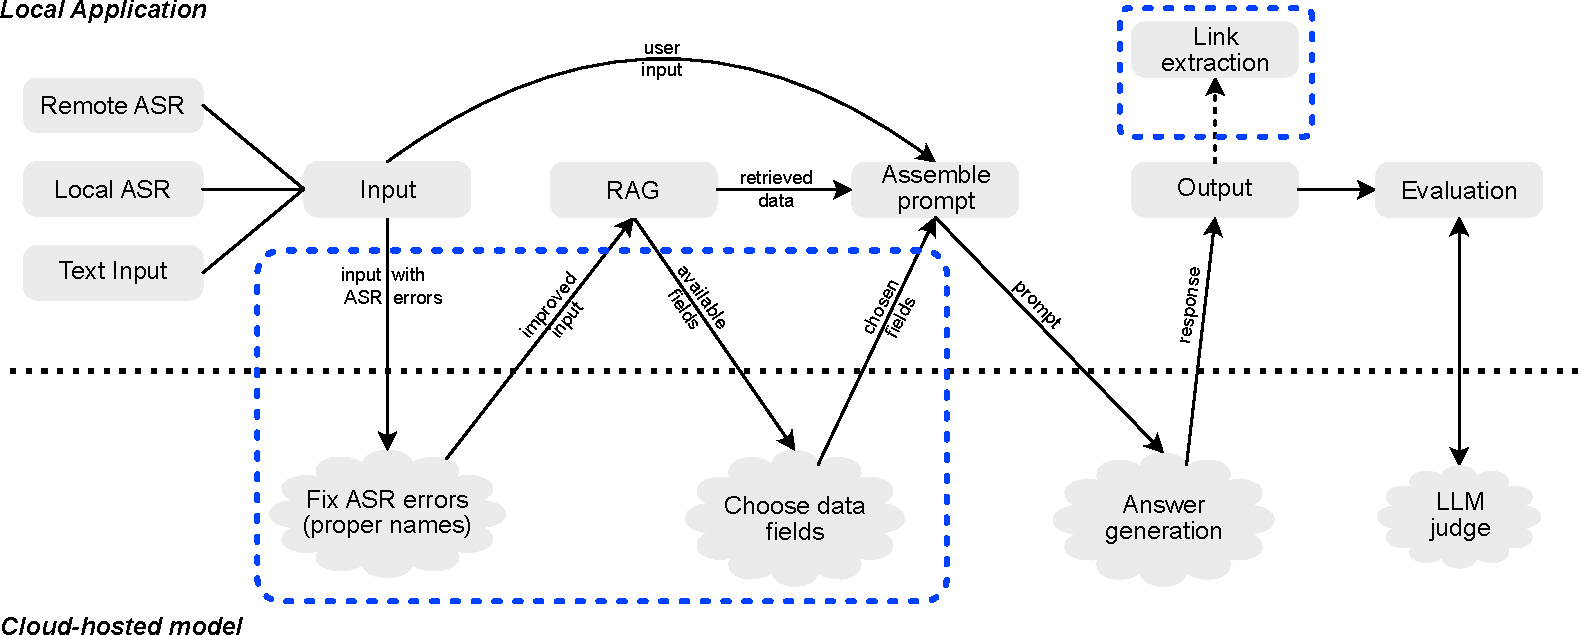
\includegraphics[width=1\linewidth]{docs/data_flow.pdf}
    \caption{Visualization of the data flow through the system's components. The parts shown within the blue boxes are planned additions for the third phase.}
    \label{fig:data_flow}
\end{figure}

The data flow graph, including currently planned additions, can be seen in~\cref{fig:data_flow}. The only usage of the model on the data that is currently implemented is the basic answer generation described in~\cref{sec:model_query}. Additional processing steps planned for the next phase include letting the model choose which data fields are needed for answering a question (see~\cref{sec:chosen_data}) and using the model to fix errors introduced during the ASR (see~\cref{sec:ASR_post_proc}). An LLM is also used in the evaluation of the system as an LLM-judge, as described in~\cref{sec:eval_quant}.



\section{Evaluation}
During the development of the MVP quality measure mainly relied on anecdotal experiences and throw-away tests. For the completion of the second phase, an automated evaluation was implemented (see~\cref{sec:eval_quant}) in order to get a baseline measurement of the system's performance that will be used to evaluate the impact that any future additions have on the response quality.

\subsection{Qualitative} \label{sec:eval_qual}
The main insight of the qualitative experiences with the system is that the MVP can work as intended under the right conditions. The qualitative evaluation was also suitable to identify the most impactful sources of errors within the system and develop initial ideas on how to improve the system's quality (see~\cref{sec:next_steps}).\\

The ASR based on a local whisper model was found to mostly correctly transcribe inputs, but especially for small models quality for German input was found to be lower compared to English input. In addition to that, the model especially struggled with German proper names, which had a high impact on the quality of retrieved documents. Due to this, the local ASR works best with commonly known words like "Mensa" instead of unknown proper names.\\

Using the remote ASR instead noticeably improved the transcription quality and also worked better, even though not perfectly, with proper names. Even though a push-to-talk implementation was chosen, the added delay for transcription is noticeable but not problematic for the mainly short inputs. The main problem of using remote ASR is that building IDs are transcribed as words instead of numbers (e.g. "Gebäude fünfzig Punkt vierunddreißig" instead of "Gebäude 50.34").\\

Another noticeable deviation from the desired behavior is that the model tends to include unnecessary information in its responses. While the correct answer to the user's question is usually returned, given that the necessary database entries are retrieved, the system tends to return all information given for the relevant building instead of just the information needed to answer the provided question.

\subsection{Quantitative} \label{sec:eval_quant}

\subsubsection{Usage of BERTScore and Limitations}
We calculated BERTScore's F1, precision and recall scores across all test cases using the method documented by the authors (see \cref{fig:overall_perf}). While the results shown in the overview sound promising, a closer inspection (see below) reveals that BERTScore is not a reliable metric for evaluating the quality of the chatbot's responses.\\

\begin{figure}[htb]
    \centering
    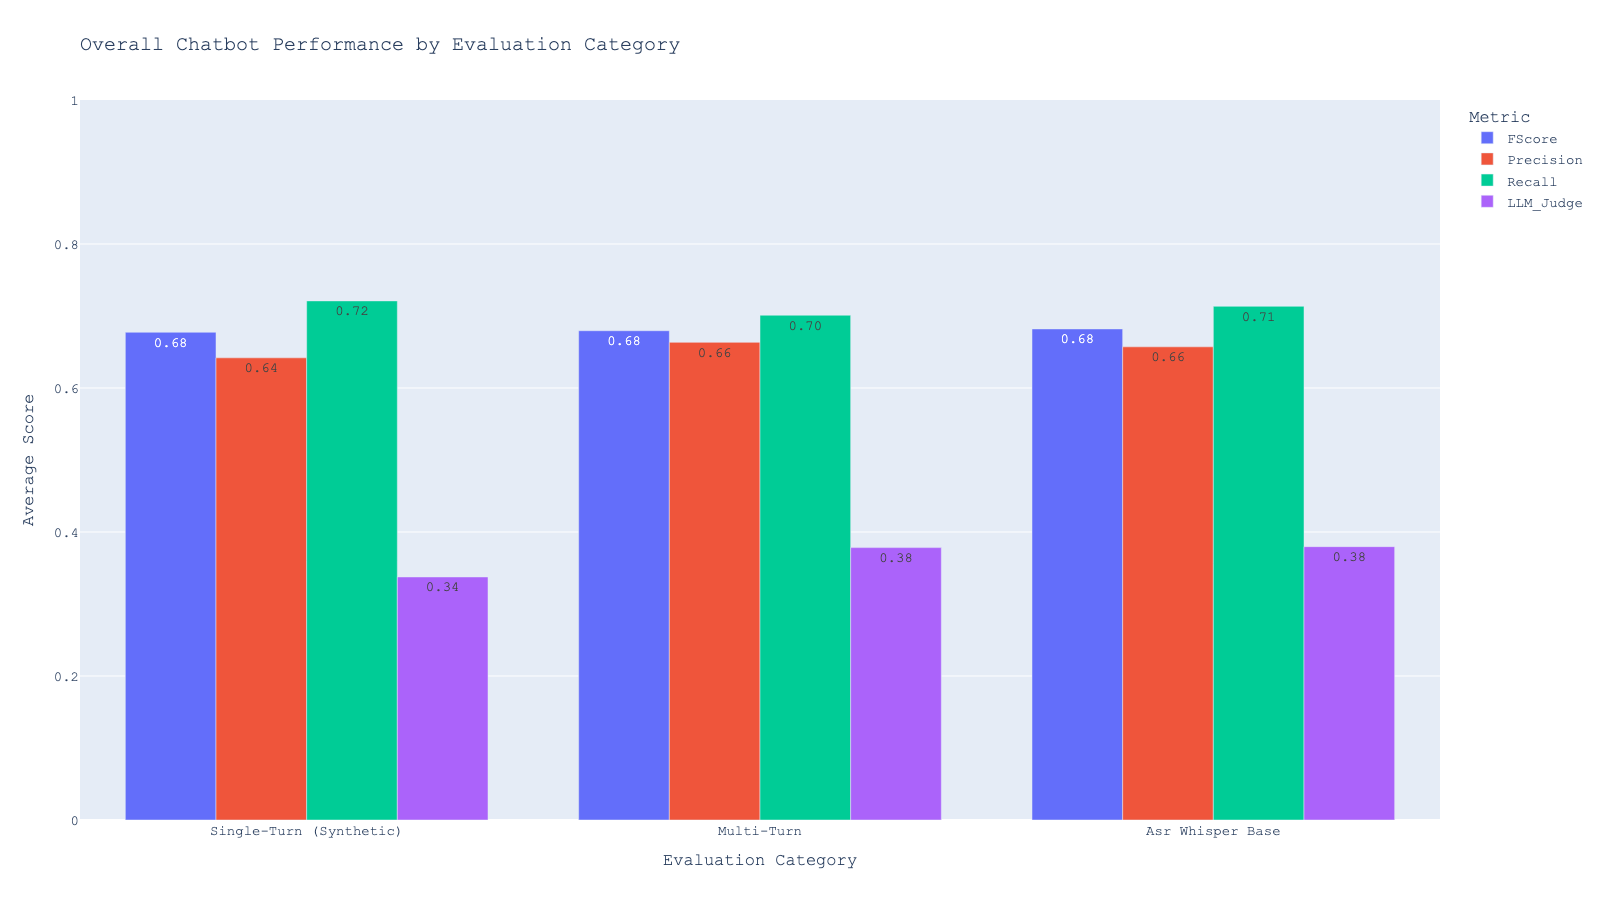
\includegraphics[width=1.0\linewidth]{docs/phase2/plots/overall_performance.png}
    \caption{Overall Chatbot Performance by Evaluation Category. FScore, Precision, and Recall are all obtained from BERTSCORE. However, these metrics paint an overly optimistic picture of the chatbot's performance, failing to depict factual inconsistencies (See \cref{tab:factual-incons}). Interestingly, there is no performance degradation in ASR. This is probably due to LLMs being very capable of understanding meaning even when faced with wrong words.}
    \label{fig:overall_perf}
\end{figure}

While it is valuable for measuring semantic similarity, BERTScore can be misleading when factual accuracy is paramount. The following example illustrates a critical weakness: BERTScore assigns a high score due to significant word overlap, despite the output being a direct and incorrect contradiction of the expected answer. This highlights the necessity of using an LLM-based judge, which correctly identifies the factual error and assigns a score of 0. A comparison of LLM-based and traditional scores can be seen in–\cref{fig:single_turn}\\

\subsubsection*{Example Case: Factual Contradiction}
\label{tab:factual-incons}
\begin{longtable}{p{0.2\textwidth} p{0.8\textwidth}}

\toprule
\textbf{Field} & \textbf{Content} \\
\midrule
\endhead
\bottomrule
\endfoot
\textbf{Input} & Ist Gebäude 210 rollstuhlgerecht? \\
\textbf{Expected Output} & Ja, das Gebäude ist rollstuhlgerecht. \\
\textbf{Actual Output} & Das Gebäude 210 ist nicht rollstuhlgerecht. \\
\midrule
\textbf{Scores} &
\begin{tabular}{@{}l@{}}
FScore: 0.87 \\
Precision: 0.87 \\
Recall: 0.86 \\
\textbf{Judge Score: 0.0}
\end{tabular}
\\
\end{longtable}

\begin{figure}[htb]
    \centering
    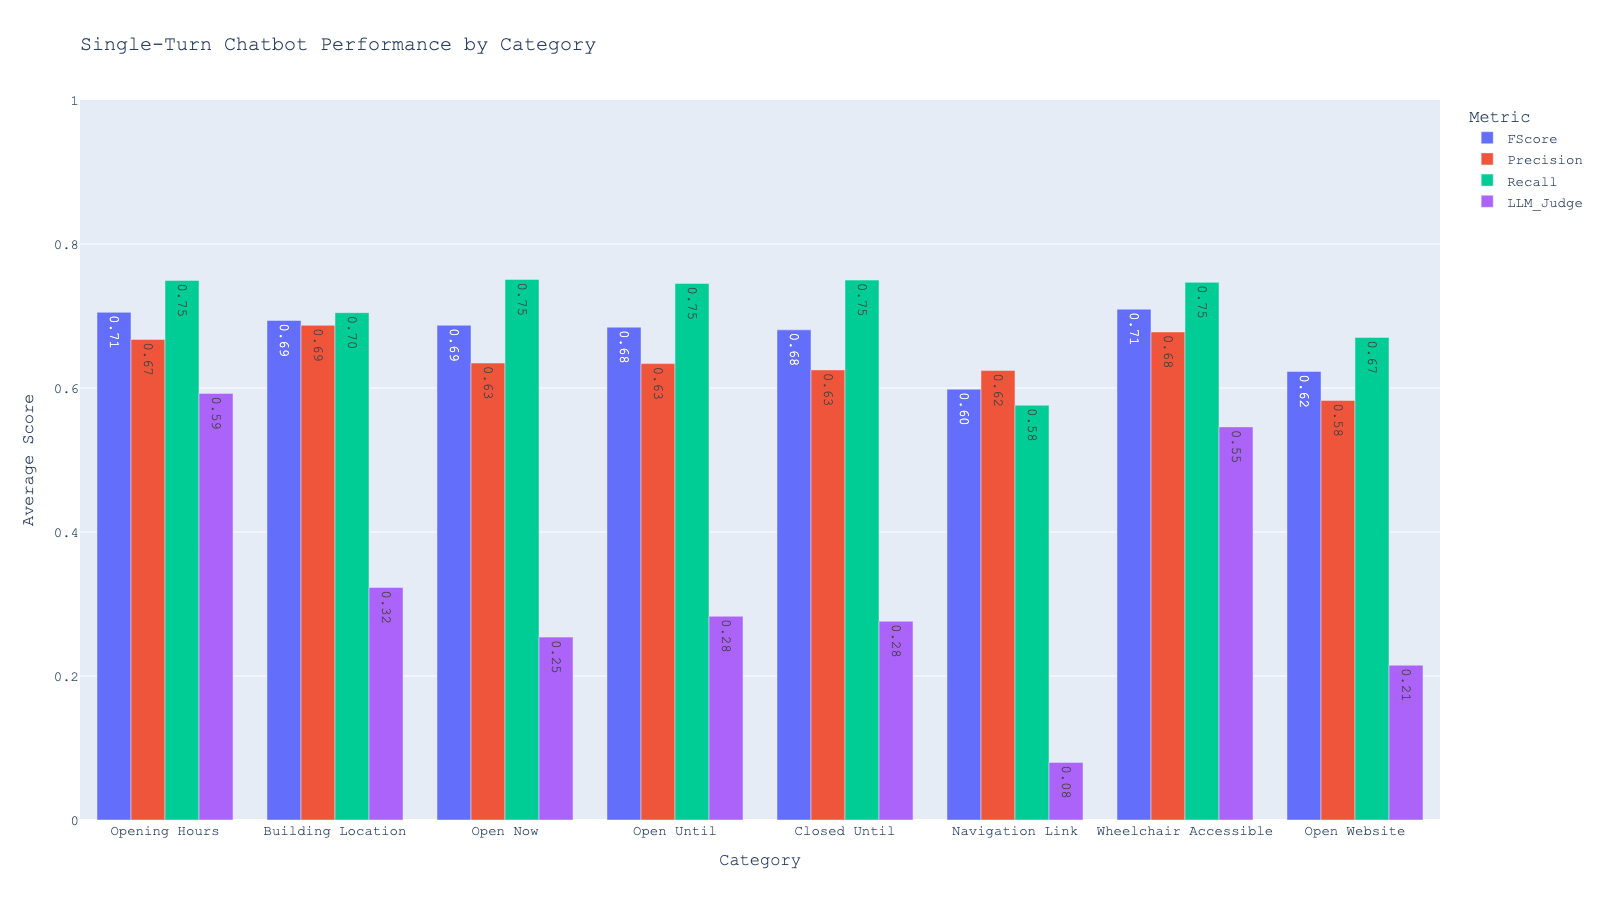
\includegraphics[width=1.0\linewidth]{docs/phase2/plots/single_turn_performance_by_category.png}
    \caption{Single Turn Chatbot Performance by Category: This diagram underscores the differences between BERTScore and LLM Judge's scores. It further demonstrates that the current system should only be seen as a baseline to improve upon. Note: All the judge's scores were averaged. Find more binary-oriented evaluation in \cref{sec:summary}.}
    \label{fig:single_turn}
\end{figure}

\subsubsection{Evaluation via Pydantic Evals' LLM Judge}
Using the LLM Judge framework provided by Pydantic that assigns a score, a binary pass/fail evaluation, and gives a reason for the score, we were able to evaluate the chatbot's responses in a systematic manner.

\subsubsection*{Challenges in LLM-based Evaluation}
The effectiveness of an LLM-as-a-judge system is highly dependent on the capability of the chosen model. An initial attempt using the institute's LLaMA 3.1 8B model revealed significant impairments in reasoning. The model failed to grasp the core requirements of the task, leading to unreliable evaluations. For instance, the prompt given to the evaluator model states that the bot has access to the underlying data if an expected output is provided. The smaller model often failed to adhere to this, incorrectly rewarding the chatbot for making excuses instead of providing the required information.

\subsubsection*{Example Case: Evaluator Model Failure}
\begin{longtable}{p{0.2\textwidth} p{0.8\textwidth}}
\toprule
\textbf{Field} & \textbf{Content} \\
\midrule
\endhead
\bottomrule
\endfoot
\textbf{Input} & Wann öffnet das Gebäude ZEISS Makerspace @ KIT? \\
\textbf{Expected Output} & Das Gebäude öffnet in 0 Tagen, 9 Stunden und 11 Minuten. \\
\textbf{Actual Output} & Das ZEISS Makerspace befindet sich im Gebäude "Kollegiengebäude am Kronenplatz" in der Kaiserstraße 89-93. Leider habe ich keine Informationen über die Öffnungszeiten des Makerspaces. Ich empfehle, auf der Website des Wirtschaftswissenschaftlichen Kollegs nachzuschauen oder direkt dort anzufragen. \\
\midrule
\textbf{Grading by Llama 3.1 8B} &
\begin{tabular}{@{}l@{}}
\textit{Reason: The output conveys the information that the chatbot does not} \\
\textit{have the current opening hours of the ZEISS Makerspace, which is} \\
\textit{consistent with the expected output.} \\
\textbf{Score: 0.8}
\end{tabular}
\\
\end{longtable}

\subsubsection*{Selecting a Capable and Reliable LLM Judge}
After determining that smaller models were insufficient, we tested a more powerful model, Mistral 24B, which was available via the Chute client's free API tier. This model demonstrated a sophisticated understanding of the evaluation rubric, capturing nuances that were previously missed. The following examples showcase its strong reasoning capabilities across different scenarios.

\subsubsection*{Trade-off Consideration}
The judge correctly penalizes the chatbot for providing related but incorrect information, while still awarding partial credit.\\

\begin{longtable}{p{0.2\textwidth} p{0.8\textwidth}}
\textbf{Input} & Wie komme ich zu Gebäude Westhochschule? \\
\textbf{Expected Output} & Mit diesem Link zu Gebäude Westhochschule führen lassen: https://www.google.com/maps/dir/?api=1\&destination=49.02041,8.36768. \\
\textbf{Output} & Das Gebäude Westhochschule liegt in der Nähe des Ehrenhofs. Die genaue Adresse lautet Fritz-Haber-Weg 7. Wenn du dich auf dem Weg dorthin befindest, kannst du die Koordinaten 49.01322, 8.41354 als Orientierungshilfe verwenden. \\
\textbf{Judge Reason} & The output does not match the expected output in meaning. The expected output should provide a link with GPS coordinates for navigation, but the output provides a general description and coordinates for orientation instead. \\
\textbf{Judge Score} & 0.5 \\
\end{longtable}

\subsubsection*{Adherence to Expected Action}
The judge understands the difference between providing information and confirming an action, correctly failing the case.\\

\begin{longtable}{p{0.2\textwidth} p{0.8\textwidth}}
\textbf{Input} & Öffne die Webseite von Gebäude Institut für Wasser und Gewässerentwicklung – Bereich Wasserwirtschaft und Kulturtechnik. \\
\textbf{Expected Output} & Ich habe die Webseite für dich in deinem Browser geöffnet. \\
\textbf{Output} & Das Institut für Wasser und Gewässerentwicklung – Bereich Wasserwirtschaft und Kulturtechnik hat seine Webseite unter https://www.iwu.kit.edu/. \\
\textbf{Judge Reason} & The output does not match the expected output in meaning. The chatbot provided useful information about the web site but did not indicate action taken. Expected output should be consistent in meaning and verbiage. \\
\textbf{Judge Score} & 0.0 \\
\end{longtable}

\subsubsection*{Handling of Additional Information}
The judge rewards the chatbot for correctly answering the core question, while slightly penalizing it for including extra, unrequested details.\\

\begin{longtable}{p{0.2\textwidth} p{0.8\textwidth}}
\textbf{Input} & Ist Gebäude Fachschaft Informatik grade geöffnet? \\
\textbf{Expected Output} & Ja, das Gebäude ist momentan geöffnet. \\
\textbf{Output} & Das Gebäude "Fachschaft Informatik" ist grade geöffnet. Laut den Öffnungszeiten ist es von Montag bis Freitag von 07:00 bis 22:30 und am Samstag von 07:00 bis 15:00 geöffnet. \\
\textbf{Judge Reason} & The output confirms the building is open, but it provides irrelevant information. The question doesn't ask for hours, but for whether the building is open, so it passes. \\
\textbf{Judge Score} & 0.75 \\
\end{longtable}

\subsubsection*{Conciseness and Semantic Equivalence}
The judge correctly identifies that a more concise answer is still factually correct and semantically equivalent, awarding a perfect score.\\

\begin{longtable}{p{0.2\textwidth} p{0.8\textwidth}}
\textbf{Input} & Wo ist Gebäude 523? \\
\textbf{Expected Output} & Das Gebäude hat die Adresse Campus Nord, Leopoldstraße, Kirchfeld, Neureut, Karlsruhe, Dettenheim, Baden-Württemberg, 76131, Deutschland. \\
\textbf{Output} & Das Gebäude 523 befindet sich auf dem Campus Nord in der Leopoldstraße in Neureut. \\
\textbf{Judge Reason} & The output conveys the same meaning as the expected output; it states the location, but slightly more concise. \\
\textbf{Judge Score} & 1.0 \\
\end{longtable}

\subsubsection{Textual Analysis of Failures}

We depict the wordcloud composed by aggregating over all reasons given by the LLM judge for all failed test cases in \cref{fig:word-cloud}. This should be taken with a grain of salt, as this is not a typical `quantitative' analysis. But there are some patterns to note, e.g. the system usually fails to convey the meaning or the right information. On the other hand, there are unnecessary details or additional information. And then, you can also see the categories surfacing again, e.g. Website, Google Maps, Building, Opening Hours.\\

\begin{figure}[htb]
    \centering
    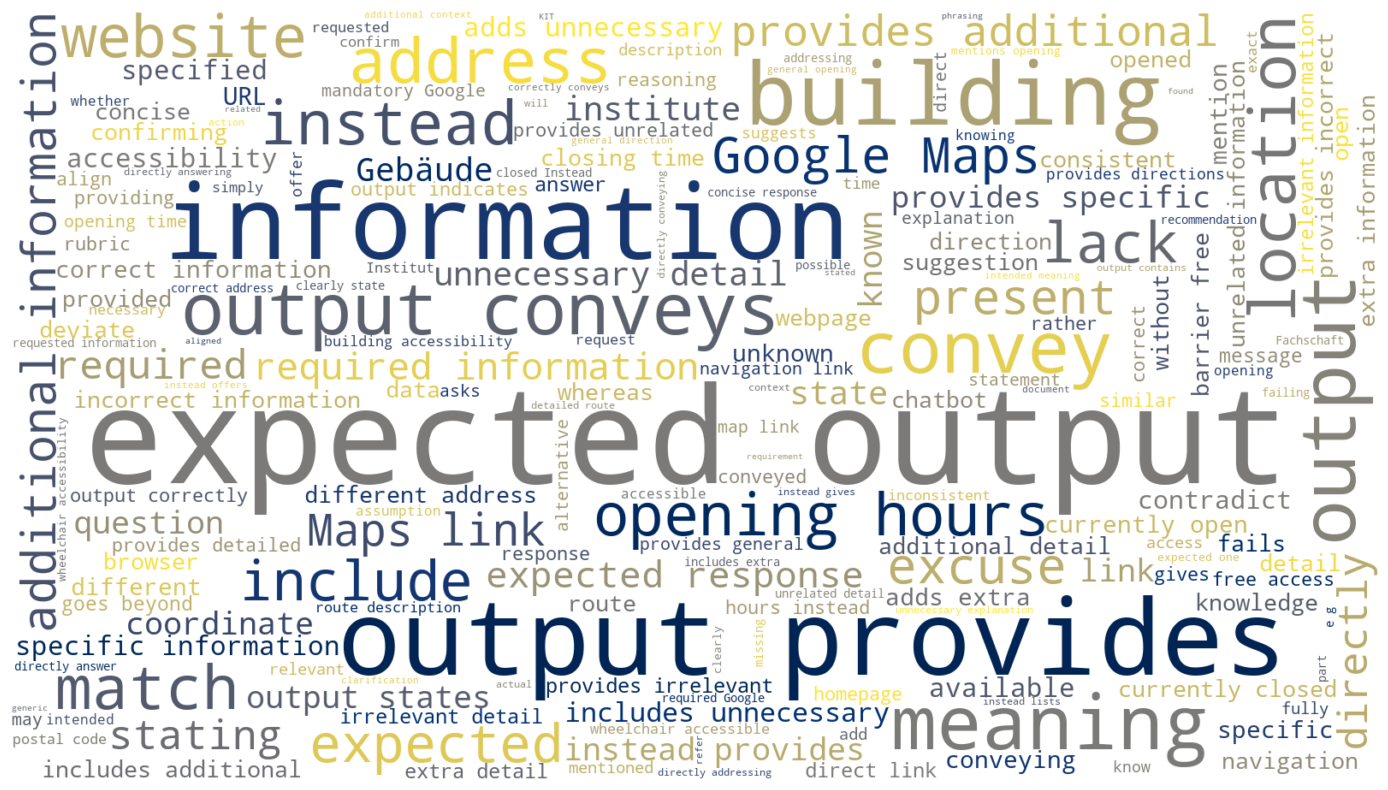
\includegraphics[width=1.0\linewidth]{docs/phase2/plots/failure_reason_wordcloud.png}
    \caption{Wordcloud of the reasons of LLM Judge for all failed test cases. Prominent themes are a lack of information, unnecessary details, and the individual single-turn categories.}
    \label{fig:word-cloud}
\end{figure}




\subsubsection{Closing thoughts on LLM Judge}

Despite its strong reasoning, the Mistral 24B model exhibited issues with consistently generating valid JSON output, which was a requirement for the automated evaluation pipeline. Consequently, for the final systematic evaluation, the Qwen3 model was selected. With a `/no\_think' directive, it provided the ideal balance of sophisticated reasoning and reliable, correctly formatted output, proving to be a robust and effective choice for the LLM judge. All in all, using LLMs to judge the output of LLMs works extremely well and is more suited than BERTScore, therefore, the following reports will only use LLM Judges to evaluate our system. This decision is underscored by the weak correlation between BERTScores and the LLM Judge's score, as can be seen in \cref{fig:heatmap}.\\

\begin{figure}[htb]
    \centering
    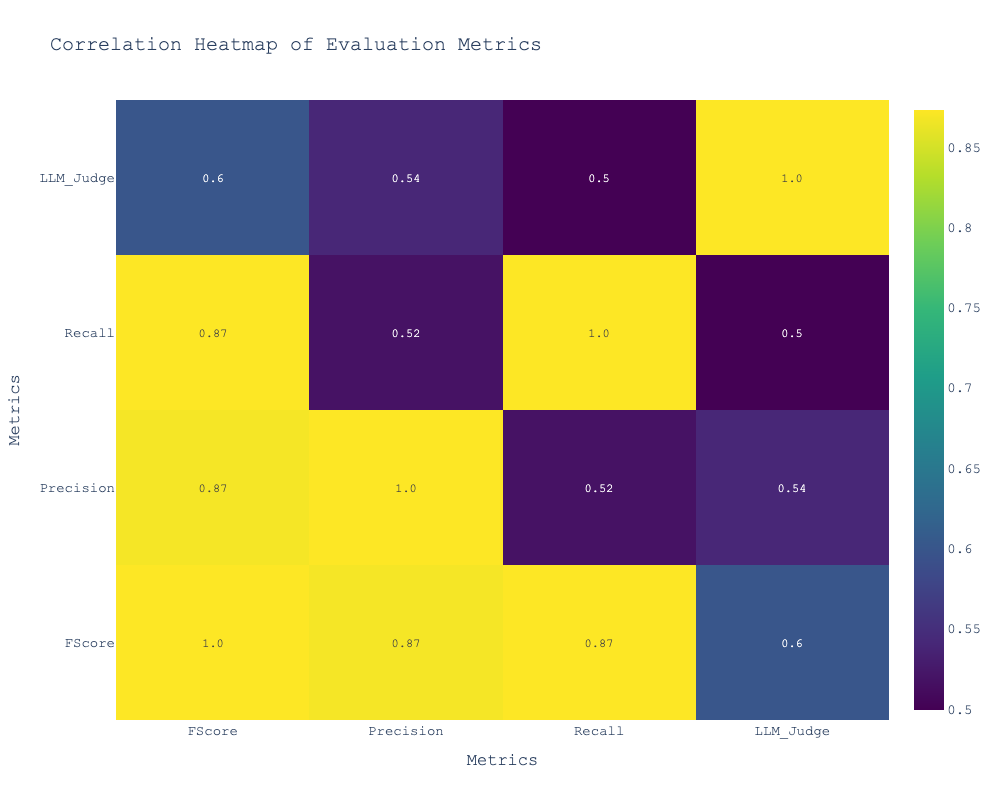
\includegraphics[width=0.8\linewidth]{docs/phase2/plots/metric_correlation_heatmap.png}
    \caption{Correlation between target metrics: LLM Judge is only weakly correlated with all BERTScore metrics.}
    \label{fig:heatmap}
\end{figure}

\subsection{Conclusion: The status quo}
\label{sec:summary}

After lots of quantitative analysis, we conclude that the current system works in some cases, i.e. for some query types and for good phrasing, s.t. the simple RAG is bringing in the correct information. Most informative proved the `LLM as a Judge' metric, as this allows us to evaluate our system's responses qualitatively for each turn but in an automated manner, thus having quantitative results as well in the end.\\

To present a clear overview, we will from now on only focus on the LLM judge's scores. Apart from obtaining the average for each category, we also forced the LLM to make a binary decision for each case: Whether the system passed the test or not. We present these clear results in \cref{tab:results}.\\


\begin{table}[!htb]
\centering
\caption{Overview of all single-turn test cases per category and the binary decision whether the answer suffices or not. This serves best as an indicator to judge the whole system's performance and can correctly pinpoint missing functionality, e.g. the `Navigation Link' feature}
\vspace{0.5cm}
\begin{tabular}{lrr}
\toprule
\textbf{Evaluation Category} & \textbf{Test Cases} & \textbf{Passing Tests} \\
\midrule
Building Location & 85 & 19 \\
Closed Until & 100 & 24 \\
Navigation Link & 50 & 0 \\
Open Now & 100 & 20 \\
Open Until & 100 & 21 \\
Open Website & 100 & 17 \\
Opening Hours & 100 & 53 \\
Wheelchair Accessible & 100 & 49 \\
\midrule
\textbf{Total} & \textbf{1828} & \textbf{533} \\
\bottomrule
\end{tabular}
\label{tab:results}

\end{table}

\newpage

\section{Next Steps} \label{sec:next_steps}
Based on the findings from this phase and the project plan developed in the last phase, there are two main courses of action for the third phase. The first is to focus on mitigating the most impactful error sources and improving the system's quality. The other is to implement the high-priority tasks defined in the first phase.

\subsection{Improve Quality} \label{sec:impr_qual}
There are three main problems negatively impacting the current system's quality. We are trying to address them in the third phase by implementing the following improvements.

\subsubsection{Alternative RAG (LlamaIndex)} \label{sec:alt_RAG}
The first ad-hoc implementation of the RAG does work under ideal conditions, but often fails to retrieve relevant documents. Using LlamaIndex as an alternative approach allows us to better adapt the retrieval to both the model in use and the kind of data we are dealing with. Despite this, we are going to keep on experimenting with combining embedding-based RAG approaches with more traditional retrieval based on regular expressions for optimal performance in the most common use cases.

\subsubsection{ASR Post-Processing} \label{sec:ASR_post_proc}
The predominant problem with both versions of the ASR is errors in the transcription of proper names, as this has a massive impact on the performance of the RAG component. In order to improve this, we are going to experiment with adding an additional model usage after the transcription and let the LLM fix as many transcription errors as possible. This might be done based on few-shot learning, aided by a list of known location names or rule-based, like changing building IDs from words to numbers.

\subsubsection{Model-Chosen Data} \label{sec:chosen_data}
To fix the issue where the model returns more information than requested by the user, we are going to add an additional model usage between the document retrieval and the answer generation. In this step, the model will pick the data fields that are needed to answer the given question and will only receive the retrieved information from those fields. By doing this, the model will have all the information needed to answer the user's question and is incapable of outputting any unnecessary information.

\subsubsection{Project Cleanup}
Because the second phase focused on "getting things to work quickly", the codebase ended up unorganized. Cleaning this up does not involve rewriting any code, since we made sure to stick to the pre-defined protocols during the implementation. However, to keep the project organized and avoid increasing organizational debt, we are going to restructure the GitHub repository and expand the documentation early in the third phase.

\subsection{Additional Features}
While the main focus in the third phase will be on improving the system's quality with the measures described in~\cref{sec:impr_qual}, we are going to try and also finish the implementation of the high-priority features defined in the first phase.

\subsubsection{Navigation Links}
Simple, throw-away tests have shown that the model is already capable of generating working links for the navigation with Google Maps, based on geo-coordinates, when specifically prompted to do so. This means that implementing the navigation links feature might be as simple as explicitly stating this functionality in the system prompt and providing some examples for few-shot learning.

\subsubsection{Current Time}
Like with navigation links, the model already has all the information needed to use the current time and date and does so when explicitly asked for it. So, including a more detailed description in the system prompt and providing some examples might be enough to encourage the intended behavior.

\subsubsection{Opening URLs}
Automatically opening URLs included in the system's responses is primarily a client-based task. For user convenience and safety, we are going to allow an opt-out of this functionality.

\end{document}
